\documentclass[runningheads]{llncs}
\usepackage{fontspec,xeCJK}
\setCJKmainfont{Noto Serif CJK SC}
\setCJKsansfont{Noto Sans CJK SC}
\usepackage{amsmath,amssymb,booktabs,graphicx,multirow}
\usepackage[hidelinks]{hyperref}
\renewcommand{\abstractname}{摘要}
\renewcommand{\keywordname}{关键词：}
\renewcommand{\figurename}{图}
\renewcommand{\tablename}{表}
\renewcommand{\refname}{参考文献}
\setlength{\emergencystretch}{1.5em}
\begin{document}
\title{Oracle 差距存在下限：\\标签获取评价中偶然性空间与可部署空间的分离}
\titlerunning{Oracle 差距存在下限}
\author{匿名作者}
\authorrunning{匿名作者}
\institute{匿名机构}
\maketitle
\begin{abstract}
标签获取基准中的 oracle 可能同时利用已实现训练结果与评价集。本文区分隐藏训练标签的完全信息价值、测试集复用，以及指定事前选择器的表现。对于固定可行集合族，我们给出不依赖分布的总体不等式及其严格的经验版本；两集合高斯表达式仅在相应假设下适用。624 个模拟状态均通过经验不等式检查。八个数据集与三类下游学习器呈现不同程度的事后机会。在三个数据集内实施随机标签翻转干预时，经验族下限均随翻转强度单调增大，而扩大候选池的效果并不一致。12 候选池的精确枚举检验了贪心近似，概率模型扰动则揭示了留出校准检验之外的敏感性。我们将交叉拟合贪心收益作为操作性基准，并明确其搜索误差与蒙特卡洛误差。延迟回放显示，DC-PRISM 可改善数量导向基准，也可能落后于信息贪心规则。由此，本文审核 oracle 差距的各部分由何种评价设计支持，而不将整个差距都解释为可实现的提升。
\keywords{主动学习 \and 评价 \and Oracle 上界 \and 偶然性不确定性 \and 风险约束获取}
\end{abstract}

\section{引言}
\label{sec:intro}
一个获取策略还能好多少？主动学习研究越来越多地用 \emph{oracle} 来回答：oracle 与任何可部署策略不同，它可以查看自己所获的标签以及评价集，从而描绘出可达到的最佳学习曲线。近期基准构造了贪心 oracle，逐步加入其\emph{实现}标签最能提升测试性能的候选~\cite{werner2023comparable,werner2024cdalbench}；还有 best-of-strategies oracle，在每一批中挑出所标注批次最有帮助的策略~\cite{huseljic2026boss}。oracle 与实用策略之间的差距随后被解读为提升空间：有研究报告，最先进的策略“明显落后于 oracle 性能，在大规模数据集上尤为明显”~\cite{huseljic2026boss}。这与让主动学习评价更可靠的更广泛努力相互呼应~\cite{luth2023navigating,ji2023randomness}。

依据实现标签做选择的 oracle 是一种\emph{事后}（ex-post）基准，它的一部分优势从构造上就不可达到：当给定协变量后结果仍是随机的，总有某个可行标签集合会“碰巧”表现最好，而只有事后才能找到它。事前与事后遗憾的区分在决策导向学习与鲁棒优化中广为人知~\cite{schutte2023robust}；在 bandit 中，期望遗憾与伪遗憾之差随各臂的噪声增大~\cite{bubeck2012regret,audibert2010regret}。但对于标签获取中的 oracle 上界，本文研究这一差距的大小，而它恰恰决定了“oracle 差距”反映的是更好策略的空间，还是仅仅是结果噪声。信贷、医疗与营销中的标签记录的是随机结果，而非近乎确定的类别，因此当标签需要通过有后果的行动来获取时，这个问题最为关键。

\paragraph{贡献。}
\begin{itemize}
\item 建立区分固定族完全信息价值、评价集复用与指定交叉拟合选择器收益的协议，并明确它们不同的识别与估计条件。
\item 给出固定族下限的不依赖分布的不等式，在 624 个状态上检查实现，并结合小池精确枚举、概率模型敏感性及数据集内标签噪声干预。
\item 在八个数据集与三类学习器上审核事后机会，将延迟回放作为独立结果核验，记录实际策略未能利用机会的情形。
\end{itemize}



\section{问题设定}
\label{sec:setting}
在第 $t$ 轮，学习者持有有标签历史 $D_t$、待反馈获取（已选择但尚未结算）的协变量 $O_t$、无标签候选池 $C_t$ 与目标协变量 $Q_t$。候选 $i$ 具有可见敞口 $e_i\ge0$ 与二元结果 $Y_i$，后者仅在获取后揭晓。策略依据可见信息 $\mathcal H_t$ 选择 $S_t\subseteq C_t$。学习效果用下游学习器（$\ell_2$ 逻辑回归、梯度提升或单隐层网络）的 Brier 分数~\cite{brier1950verification}度量；$L(S;Y)$ 为其在 $D\cup O\cup S$ 上拟合后的测试损失，其中 $Y$ 汇集 $O$ 与 $S$ 的隐藏训练结果。

\paragraph{风险预算。}获取一个标签是一次有敞口的行动，例如放贷机构批准申请人以观察其还款~\cite{lakkaraju2017selective,wei2021selective}。给定风险分数 $q_i$、$\ell=\log(1/\alpha)$，当 $q\le\frac12$ 时 $\phi(q)=q(1-q)$，否则为 $\frac14$，可行集合满足
\begin{equation}
 R_\alpha(S)=\sum_{i\in S}e_iq_i+\Big(2\ell\sum_{i\in S}e_i^2\phi(q_i)\Big)^{1/2}+\frac{\ell}{3}\max_{i\in S}e_i\le B_t,
 \label{eq:envelope}
\end{equation}
这是一个次伽马界~\cite{boucheron2013concentration}：在条件独立且 $p_i\le q_i$ 时，实际不利敞口超过 $R_\alpha(S)$ 的概率至多为 $\alpha=0.1$。我们的分数 $q_i$（拟合 logit 的 40 个 Laplace 抽样经 Wilson 平移~\cite{wilson1927probable}后的高分位数）不保证 $p_i\le q_i$，因此式~\eqref{eq:envelope} 是所有策略共享的操作性可行域。预算 $B_t$ 取风险最低的 $k$ 个候选之包络的 $1.03$ 倍（除非另行说明，$k=6$）；\emph{数量参照} $M_K$ 为最大的可行集合，候选不超过 16 个时穷举，否则采用按敞口分层的搜索，其在 1{,}408 个状态中的 1{,}320 个认证了基数，其余 88 个状态经后续精确搜索也认证了数量最优。对于没有天然敞口的基准数据集，令 $e_i=1$。

\section{分解 Oracle 差距}
\label{sec:protocol}
\paragraph{族 oracle。}固定 $\mathcal H$ 以及由可见信息构造、包含 $M=M_K$ 的可行集合族 $\mathcal F$。记 $\bar L$ 为积分掉测试标签噪声后的测试损失，
\begin{align}
 H_{\mathrm{post}}&=\mathbb E\big[\bar L(M;Y)-\min_{S\in\mathcal F}\bar L(S;Y)\mid\mathcal H\big],\\
 H_{\mathrm{pre}}&=\mathbb E[\bar L(M;Y)\mid\mathcal H]-\min_{S\in\mathcal F}\mathbb E[\bar L(S;Y)\mid\mathcal H].
\end{align}
$H_{\mathrm{post}}$ 是看到隐藏训练标签后再挑最佳集合的 oracle 的领先；$H_{\mathrm{pre}}$ 是最佳固定选择的领先。二者之差，即\emph{偶然性下限} $F=H_{\mathrm{post}}-H_{\mathrm{pre}}\ge0$（因为 $\mathbb E\min\le\min\mathbb E$），是选择限制在 $\mathcal F$ 内的策略无法弥合的部分，它就是关于训练结果的完全信息期望值~\cite{howard1966information}。对限制在该族内、期望收益为 $\Gamma_\pi$ 的策略，$H_{\mathrm{post}}-\Gamma_\pi=F+(H_{\mathrm{pre}}-\Gamma_\pi)$，只有第二项即\emph{选择差距}可以被弥合。

\paragraph{贪心基准诊断。}基准利用已实现标签与评价集贪心选择批次~\cite{werner2023comparable,werner2024cdalbench}。将测试记录拆为 $T_1,T_2$。令 $G_{\rm rep}$ 为在 $T_1$ 选择并评分的平均收益，$G_{\rm hold}$ 为同一选择器在 $T_2$ 的收益；$G_{\rm cf}$ 为在一个训练标签重复样本库上按平均 $T_1$ 损失选择、在另一独立样本库上用 $T_2$ 评分的贪心规则收益，交换两库后平均。则
\[
G_{\rm rep}=(G_{\rm rep}-G_{\rm hold})+(G_{\rm hold}-G_{\rm cf})+G_{\rm cf}.
\]
这是一条记账恒等式。第一项诊断评价集复用，第二项是\emph{贪心残差}，同时包含搜索与有限模拟效应。只有在选择器优化同一候选族，且目标与评价分布一致等条件下，它才对应固定族下限。因此，本文不将该残差认定为不可消除下限，也不将 $G_{\rm cf}$ 称为最优可部署价值。

\paragraph{有效的固定族不等式。}记 $d_S=\bar L(M;Y)-\bar L(S;Y)$、$\mu_S=\mathbb E d_S$，令 $b$ 最大化 $\mu_S$，$r$ 为另一集合。族下限为 $F=\mathbb E\max_S d_S-\max_S\mu_S$。逐点比较及中心化可得
\begin{equation}
\mathbb E(d_r-d_b)_+\ \leq F\ \leq\mathbb E\max_S(d_S-\mu_S).\label{eq:two}
\end{equation}
因为 $\max_S d_S-d_b\ge(d_r-d_b)_+$，且 $\max_S d_S\le\max_S\mu_S+\max_S(d_S-\mu_S)$。以同一经验分布替换期望与均值后，样本不等式严格成立，即使 $b,r$ 由该样本选择亦然；但这不提供总体 $F$ 的置信覆盖。若中心化收益联合高斯，则允许任意相关性，并有 $F\le\max_S\sigma_S\sqrt{2\log|\mathcal F|}$。若 $d_b-d_r$ 为均值 $\Delta$、标准差 $s$ 的正态变量，下界表达式为 $s\varphi(\Delta/s)-\Delta\Phi(-\Delta/s)$。正态性是额外建模假设；独立正态构造不是普适上界。

\paragraph{估计与模型替代。}已知 $p$ 时，以公共随机数生成训练标签重复样本。在固定族中，最大化估计平均收益所得 $H_{\rm pre}$ 估计在期望上偏高；在一库选择、另一库评估，则估计有限样本选择器的期望价值，该值不超过 $H_{\rm pre}$。两者均不构成单次有限样本的确定性夹逼。真实数据用不相交辅助记录拟合的梯度提升模型提供 $\hat p$，记录的测试标签保持固定，因此评价以该测试集与概率模型为条件。模拟与记录结果的事后差距比较仅检验模型的一个泛函，不能完全识别下限。逐状态对带噪声的策略收益估计取最大值，会进一步引入选择乐观性；此类事后最大值属于敏感性汇总，不是可实现价值的认证下界。

\section{被评价的策略}
\label{sec:policy}
所有策略共享状态、$q$、预算与式~\eqref{eq:envelope}。\emph{Safe-MinRisk} 返回 $M_K$；\emph{固定数量}按点价值选取 $K$ 的固定比例；\emph{Fisher-cost} 按单标签方差下降与敞口之比装填。另有四个规则贪心装填直到没有可行候选：\emph{Random}、\emph{Uncertainty}~\cite{lewis1994sequential}、对 $\operatorname{tr}(F_Q(H_{D+O}+A_S)^{-1})$ 的 \emph{BAIT-greedy}~\cite{ash2021fishing}，以及对目标加权代理
\begin{equation}
 V_\theta(S)=\operatorname{tr}\big[W_Q\{H_{D+O}^{-1}-(H_{D+O}+A_S)^{-1}\}\big]\label{eq:value}
\end{equation}
做贪心的 \emph{TargetVar-greedy}，其中 $H_{D+O}$ 为历史与待反馈协变量的逻辑 Fisher 信息，$A_S$ 为 $S$ 的 Fisher 信息，$W_Q$ 按 Brier 敏感度对目标方向加权~\cite{yu2006transductive,bickfordsmith2023prediction}。\emph{Proxy-argmax} 在评估族上取 $\arg\max V_{\hat\theta}$。\emph{DC-PRISM} 是为带待反馈结果的风险约束获取设计的保守策略：它在以 $M_K$ 为锚的族上、于 20 个 Laplace 参数抽样~\cite{mackay1992practical}下评估式~\eqref{eq:value}，以 $\tanh\{(V_m(S)-V_m(M_K))/2.5V_m(M_K)\}$ 的 0.2 分位数减去数量惩罚 $0.22(K-|S|)_+/K$ 为每个集合打分，除非最佳得分超过 $0.08$，否则返回 $M_K$。24 个候选时一次选择约需 50\,ms。这里所有信息代理都由逻辑模型推出。

\section{协议的验证}
\label{sec:validation}
\paragraph{研究设置。}每项研究在运行前固定状态、种子、比较族以及 $5\times10^{-4}$ Brier 的实质效应阈值，协议与代码在版本库中冻结；我们报告配对均值、95\% Bonferroni 同时区间与 Holm 校正检验~\cite{holm1979simple}。所有数值单位为 $10^{-3}$ Brier。数据集包括：四个信贷数据集（HMEQ、LendingClub、PPDai、UCI Credit~\cite{sasHMEQ,lendingclubSource,ppdaiSource,he2018ensemble,yeh2009comparison}）、以住院天数为敞口的 30 天再入院~\cite{strack2014impact}、银行营销认购、Spambase，以及 USPS 手写数字（$\ge5$ 对 $<5$），后者分别以原始像素与 10 个主成分表示。每个状态是延迟回放的第一轮，含 68 个历史标签、14 个待反馈记录与 24 个候选；候选随机抽取（\emph{自然}流），对信贷与再入院数据还另有\emph{工程}流，按协变量排序提供低风险、与待反馈对齐、互补与尾部候选。受控世界与\emph{半合成}状态（真实协变量、由已知 logit 生成结果）提供已知的 $p$。

\paragraph{估计概率能复原已知概率下的结果。}在 512 个半合成状态上，用在以真实 $p$ 标注的辅助记录上拟合的梯度提升 $\hat p$，其估计相对已知 $p$ 协议的偏差在 96 项检查（8 组 $\times$ 12 个量）中有 95 项落在 $\pm0.5$ 以内；$H_{\mathrm{post}}$、$H_{\mathrm{pre}}$、下限与主要策略收益的平均偏差至多 $0.20$，$H_{\mathrm{pre}}$ 的状态层面相关为 $0.73$--$0.95$。逻辑回归 $\hat p$ 在真值为非线性时把 $H_{\mathrm{pre}}$ 低估 $0.26$--$0.28$，因此估计需要灵活的 $\hat p$。

\paragraph{记录结果检查与敏感性。}置信区间包含零并不证明一致。返修采用显示单位下 $0.5$ 的等价界限。逻辑回归与梯度提升学习器的汇总检查支持等价，但 16 个单独数据集与学习器格子中仅两格证明等价，神经学习器汇总也未通过。在另 192 个贪心校准状态中，报告差距的汇总差异 90\% 区间为 $[-0.089,0.416]$，落在等价界内；留出差距区间 $[-0.138,0.513]$ 则越界。已知概率的扰动检查中，未扰动模型的平均下限偏差约 $-0.04$，但调整概率锐度使偏差改变约 $0.5$--$0.8$。不相交拟合很重要，却不能证明对概率模型误设稳健。

\paragraph{候选族敏感性。}为每个族加入 64 个随机可行集合（从 22--27 个扩大到 81--88 个），估计的可部署占比 $H_{\mathrm{pre}}/H_{\mathrm{post}}$ 基本不变：受控世界中，在 2 到 80 的每种子族大小下都为 80--83\%；半合成分支为 6--38\%，且随 $|\mathcal F|$ 略升而非下降。

\section{发现}
\label{sec:findings}
\paragraph{留出选择使贪心基准差距缩小。}表~\ref{tab:known} 保留原始交叉拟合贪心估计，各列实现第~\ref{sec:protocol} 节的记账恒等式；其中残差包含近似误差，不是固定族 $F$。半合成状态中，相对最好固定策略的报告领先为 $6.9$，交叉拟合贪心领先约为零。记录结果状态中的表观领先也明显缩小。这证明评价设计会影响差距，但不能证明被扣除的整个部分都不可消除。

\begin{table}[t]
\caption{风险预算下的基准贪心 oracle，逻辑回归学习器（$\times10^{-3}$ Brier）。报告差距 $=$ 测试集复用 $+$ 贪心残差 $+$ 交叉拟合贪心收益。最后一列：相对最佳固定实用策略的领先，即报告值 $\to$ 去除复用与残差后的值。}
\label{tab:known}
\centering\scriptsize
\setlength{\tabcolsep}{3.5pt}
\begin{tabular}{lrrrrrr}
\toprule
设定 & 状态数 & 报告 & 复用 & 残差 & 可部署 & 相对最佳的领先 \\
\midrule
受控世界 & 64 & 29.5 & 4.5 & 3.5 & 21.5 & 15.8$\to$7.8 \\
半合成（已知 $p$） & 256 & 7.2 & 2.9 & 3.9 & 0.3 & 6.9$\to$0.0 \\
信贷，工程流 & 128 & 8.0 & 0.6 & 4.1 & 3.3 & 6.7$\to$2.0 \\
信贷，自然流 & 128 & 3.4 & 0.8 & 1.7 & 0.9 & 3.2$\to$0.6 \\
再入院，两种流 & 64 & 2.3 & 0.3 & 1.4 & 0.5 & 2.0$\to$0.3 \\
\bottomrule
\end{tabular}
\end{table}

\paragraph{噪声排序与直接干预。}原跨数据集研究登记了噪声指标与贪心残差占比的关系（表~\ref{tab:gradient}）。其解释依赖事前基准：采用事后增强的比较器后，逻辑回归秩相关变为 $0.93$，神经学习器为 $0.52$（$p=0.15$），后者不再构成明确的跨数据集证据。另一项登记干预在 HMEQ、Bank Marketing 和 USPS 内，以 $0,0.1,0.2,0.3$ 的概率随机翻转标签，每个剂量、每个数据集有 16 个状态。三个数据集的经验固定族下限均单调增加（图~\ref{fig:floor}b）。这支持指定模拟中对随机标签污染的响应，不构成自然标签噪声下的普适单调规律。

\begin{table}[t]
\caption{沿标签噪声梯度的基准 oracle（自然流；逻辑回归每个数据集 48 个状态，神经网络 32 个；$\times10^{-3}$ Brier）。噪声：$\hat p(1-\hat p)$ 的均值。复用与残差：占报告差距的百分比。领先：相对最佳固定策略，报告值 $\to$ 可部署值。}
\label{tab:gradient}
\centering\scriptsize
\setlength{\tabcolsep}{2.6pt}
\begin{tabular}{lrrrrrrrrr}
\toprule
& & \multicolumn{4}{c}{逻辑回归学习器} & \multicolumn{4}{c}{神经网络学习器（MLP）} \\
\cmidrule(lr){3-6}\cmidrule(lr){7-10}
数据集 & 噪声 & 差距 & 复用 & 残差 & 领先 & 差距 & 复用 & 残差 & 领先 \\
\midrule
USPS，原始像素 & 0.036 & \multicolumn{4}{c}{--} & 18.7 & 32 & 10 & 15.9$\to$8.0 \\
Spambase & 0.054 & 7.5 & 32 & 16 & 5.1$\to$1.5 & 14.1 & 25 & 29 & 11.4$\to$3.8 \\
USPS，10 个主成分 & 0.065 & 10.8 & 12 & 13 & 7.7$\to$5.0 & 16.6 & 23 & 29 & 15.0$\to$6.4 \\
再入院 & 0.081 & 1.3 & 29 & 66 & 1.1$\to$$-$0.1 & 4.8 & 23 & 54 & 4.0$\to$0.3 \\
银行营销 & 0.091 & 4.5 & 15 & 39 & 4.1$\to$1.7 & 11.9 & 34 & 29 & 10.3$\to$2.8 \\
HMEQ & 0.101 & 3.4 & 15 & 42 & 3.0$\to$1.0 & 7.8 & 26 & 39 & 7.2$\to$2.1 \\
PPDai & 0.108 & 2.8 & 17 & 60 & 2.7$\to$0.5 & 10.4 & 20 & 38 & 9.1$\to$3.0 \\
UCI Credit & 0.136 & 3.4 & 15 & 67 & 3.2$\to$0.4 & 8.2 & 47 & 38 & 7.8$\to$0.8 \\
LendingClub & 0.144 & 2.7 & 8 & 79 & 2.8$\to$0.4 & 8.5 & 39 & 53 & 8.6$\to$0.7 \\
\bottomrule
\end{tabular}
\end{table}

\paragraph{界限、搜索与规模检查。}修正后的经验上下界在全部 624 个返修状态中成立。其有效性来自代数，因此这项检查验证实现，不是新的总体置信保证。负相关、偏态与重尾压力测试否定了原独立正态捷径。12 候选池中穷举全部可行集合（平均约 730 个）得到与贪心近似接近的汇总诊断：平均残差差异约 $-0.02$，事前收益差异约 $0.01$，单位同表格。这仅检查相应规模的近似。候选池为 24、48、96 时，下限变化具有异质性，不能据此宣称大池近似保证。

\begin{figure}[t]
\centering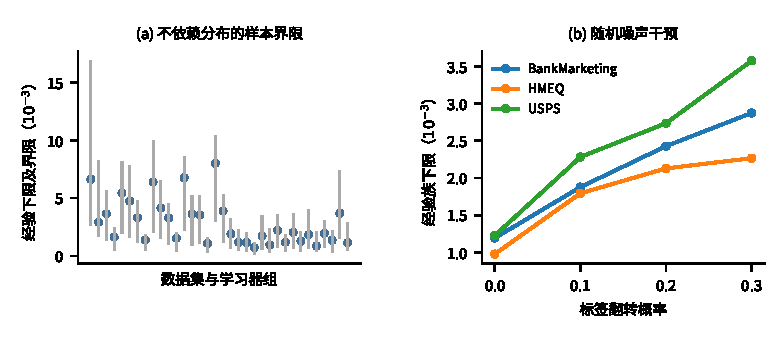
\includegraphics[width=\linewidth]{figures/fig_predict.pdf}
\caption{修正诊断。(a) 各组经验下界、下限与上界，共覆盖 624 个状态；验证经验恒等关系，不提供总体覆盖。(b) 数据集内随机标签翻转：四种剂量下的经验族下限，每个剂量、每个数据集 16 个状态；连线连接描述性均值。}
\label{fig:floor}
\end{figure}

\paragraph{预算敏感性是经验结果。}增大预算可以扩大可行族，但 $F=H_{\rm post}-H_{\rm pre}$ 是两个变化量之差，不必增大。在登记预算实验中，目标数量由 3 变为 6、12 时，八个数据集的经验族下限均增大，配对平均增加 $0.74$，区间为 $[0.67,0.82]$，单位同表格（图~\ref{fig:budget}）。这是所测分布与学习器的结果，并非式~\eqref{eq:two} 的推论。

\begin{figure}[t]
 \centering
 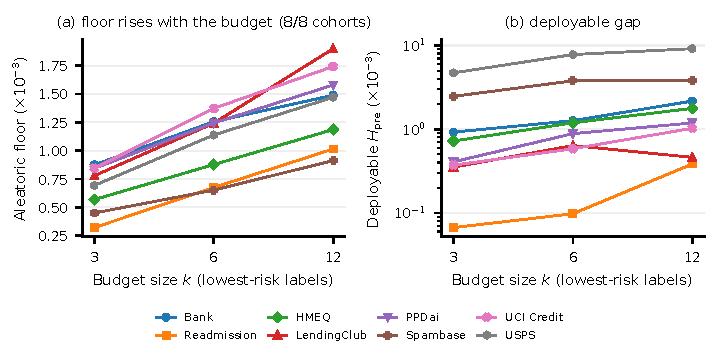
\includegraphics[width=\linewidth]{figures/fig_budget.pdf}
 \caption{风险预算作为杠杆（逻辑回归学习器，每个数据集每档预算 32 个状态）。预算按风险最低的 $k$ 个候选确定。(a) 偶然性下限在全部八个数据集上单调上升。(b) 可部署差距（对数尺度）的变化远不如下限一致。}
 \label{fig:budget}
\end{figure}

\paragraph{谁能弥合事前选择器估计收益取决于学习器。}表~\ref{tab:who} 在相同的真实标签状态上，报告两种学习器下的事前选择器估计收益与三种策略的收益。在逻辑回归学习器下，由该模型推出的信息代理在事前选择器估计收益最大的地方弥合了其中很大一部分：在工程流 HMEQ 与 LendingClub 上，TargetVar-greedy 与 Proxy-argmax 拿到了 $3.2$--$3.4$ 中的 $1.5$--$2.1$（在另一批独立的 128 种子研究中为 $4.9$--$5.7$ 中的 $2.5$--$2.9$，且 DC-PRISM 在 LendingClub 上落后 TargetVar-greedy $2.8$，区间 $[0.0,5.6]$）。在梯度提升学习器下，事前选择器估计收益仍有 $0.7$--$2.7$，DC-PRISM 的选择差距在八个信贷格子中有六个达到实质水平，但没有任何策略拿到超过 $0.65$：与逻辑模型匹配的代理无法迁移到梯度提升学习器。在再入院数据上，事前选择器估计收益很小（$0.7$--$0.9$），各策略之间没有决定性差异。

\begin{table}[t]
\caption{真实标签状态上的可部署差距 CF gain（交叉拟合）与相对 $M_K$ 的收益（信贷每格 64 个状态，再入院每格 128 个；$\times10^{-3}$ Brier）。DC：DC-PRISM；TV：TargetVar-greedy；Proxy：Proxy-argmax。}
\label{tab:who}
\centering\scriptsize
\setlength{\tabcolsep}{3pt}
\begin{tabular}{lrrrrrrrr}
\toprule
& \multicolumn{4}{c}{逻辑回归学习器} & \multicolumn{4}{c}{梯度提升学习器} \\
\cmidrule(lr){2-5}\cmidrule(lr){6-9}
状态 & CF gain & DC & TV & Proxy & CF gain & DC & TV & Proxy \\
\midrule
HMEQ，工程 & 3.21 & 0.09 & 1.51 & 1.64 & 2.32 & 0.48 & 0.15 & 0.44 \\
LC，工程 & 3.37 & 1.15 & 2.01 & 2.12 & 1.53 & 0.05 & $-$0.42 & $-$0.19 \\
PPDai，工程 & 1.87 & 0.37 & 0.04 & 0.07 & 1.18 & 0.33 & 0.17 & 0.11 \\
UCI，工程 & 0.16 & $-$0.08 & $-$0.08 & $-$0.08 & 0.84 & 0.36 & 0.42 & 0.34 \\
HMEQ，自然 & 1.26 & $-$0.22 & 0.21 & 0.12 & 2.66 & 0.24 & 0.64 & 0.65 \\
LC，自然 & 0.91 & $-$0.04 & $-$0.20 & $-$0.05 & 1.45 & $-$0.07 & 0.04 & $-$0.04 \\
PPDai，自然 & 0.59 & 0.10 & $-$0.17 & 0.02 & 1.17 & $-$0.03 & $-$0.18 & $-$0.10 \\
UCI，自然 & 0.92 & 0.07 & 0.19 & 0.32 & 1.60 & 0.03 & 0.13 & 0.08 \\
再入院，工程 & 0.84 & 0.09 & $-$0.14 & $-$0.34 & 0.92 & $-$0.01 & $-$0.25 & $-$0.28 \\
再入院，自然 & 0.67 & 0.06 & 0.30 & 0.36 & 0.72 & 0.00 & $-$0.10 & $-$0.07 \\
\bottomrule
\end{tabular}
\end{table}

\paragraph{受控世界中的 DC-PRISM。}在围绕方向性待反馈信息构造的世界中，83\% 的事后提升空间估计为事前价值，DC-PRISM 拿到了其中三分之二：它相对 Safe-MinRisk 的收益为 $12.2$，区间 $[7.6,16.8]$，所用标签为 $3.1$ 个而非 6 个；在我们尝试的全部十二种生成器变体中（待反馈重叠、风险—信息耦合、无误设尾部、48 个候选且 $K=12$），该收益都保持实质水平（$10.8$--$31.4$）。共同族消融把这一收益归因于在锚定族上评估的代理（仅 Proxy-argmax 就收益 $13.1$，区间 $[6.1,20.2]$）；保守层只多出未经证实的 $3.0$（区间 $[-0.2,6.2]$），而考虑待反馈信息的作用在我们的证据中未被单独分离出来。

\section{结局核验：延迟回放}
\label{sec:replay}
协议评价的是单轮。为检验其排序在动态过程中是否成立，我们进行了十轮回放（探索标签一轮后到达，常规标签两轮后到达；ALC-Brier 为十个轮初分数的平均），每个信贷格子 512 个新种子、每个再入院流 256 个，种子数依据前一批的方差预先登记。表~\ref{tab:replay} 报告独立的动态比较。在信息贪心规则拿到了可部署差距而 DC-PRISM 没有的地方（工程流 HMEQ 与 LendingClub），DC-PRISM 显著不如 Fisher-cost、BAIT-greedy 与 TargetVar-greedy（$2.5$--$3.8$）；在其相对数量参照的收益显著之处，它胜过 Safe-MinRisk 与固定数量（$2.2$--$3.1$）；在工程流再入院上，它胜过 BAIT-greedy 与 TargetVar-greedy（$1.3$、$1.4$）；在可部署差距很小之处（自然流、工程流 UCI），没有任何比较达到实质水平。实际不利敞口超过包络的次数：信贷每个策略 40{,}960 个采集回合中为 0--4 次，再入院 5{,}120 个回合中为 0 次。

\begin{table}[t]
\caption{延迟回放：对照策略减 DC-PRISM 的 ALC-Brier（$\times10^{-3}$；正值有利于 DC-PRISM；加粗为在登记检验族下达到实质水平）。}
\label{tab:replay}
\centering\scriptsize
\setlength{\tabcolsep}{2.4pt}
\begin{tabular}{lrrrrrrrrrr}
\toprule
& \multicolumn{4}{c}{信贷，工程流} & \multicolumn{4}{c}{信贷，自然流} & \multicolumn{2}{c}{再入院} \\
\cmidrule(lr){2-5}\cmidrule(lr){6-9}\cmidrule(lr){10-11}
对照策略 & HMEQ & LC & PPDai & UCI & HMEQ & LC & PPDai & UCI & 工程 & 自然 \\
\midrule
Safe-MinRisk & \textbf{2.4} & 0.4 & \textbf{3.1} & $-$0.1 & 0.2 & 0.2 & 0.4 & 0.1 & 0.0 & 0.2 \\
固定数量 & \textbf{2.2} & 0.4 & \textbf{2.4} & $-$0.1 & 0.1 & 0.1 & 0.3 & 0.0 & 0.4 & 0.2 \\
Random & 0.6 & $-$0.3 & \textbf{2.4} & 0.0 & 0.3 & 0.5 & 0.6 & 0.4 & 0.8 & 0.5 \\
Uncertainty & 0.5 & 1.4 & 0.7 & 0.0 & 0.4 & 0.4 & 0.1 & 0.1 & 0.4 & 0.0 \\
Fisher-cost & \textbf{$-$3.8} & \textbf{$-$3.3} & 0.8 & $-$0.1 & $-$0.3 & $-$0.1 & 0.1 & $-$0.1 & 1.0 & 0.0 \\
BAIT-greedy & \textbf{$-$3.6} & \textbf{$-$2.7} & 0.3 & 0.1 & $-$0.2 & 0.0 & 0.1 & 0.0 & \textbf{1.3} & 0.1 \\
TargetVar-greedy & \textbf{$-$3.5} & \textbf{$-$2.5} & 0.0 & 0.0 & $-$0.2 & $-$0.1 & 0.0 & $-$0.1 & \textbf{1.4} & 0.0 \\
\bottomrule
\end{tabular}
\end{table}

\section{相关工作}
\label{sec:related}
\paragraph{主动学习的评价。}近期研究表明，主动学习的收益在现实评价下很脆弱~\cite{luth2023navigating}，对不受控的随机性敏感~\cite{ji2023randomness}，并在不同领域间不一致~\cite{werner2023comparable,werner2024cdalbench}，并用 oracle 界定可达到的性能~\cite{werner2024cdalbench,huseljic2026boss}。Werner 等指出其贪心 oracle 会在测试集上过拟合~\cite{werner2023comparable}。我们量化了这种复用，并补充了去除复用后仍然存在的偶然性成分。

\paragraph{遗憾概念与不确定性。}决策导向学习与鲁棒优化区分事前与事后遗憾~\cite{schutte2023robust}；在 bandit 中，期望遗憾比伪遗憾多出一个噪声项~\cite{bubeck2012regret,audibert2010regret}；Brier 分数等 proper scoring rule 能把偶然性与认知不确定性分开~\cite{hofman2024quantifying}；在带噪声的估计中挑选最优会产生乐观偏差~\cite{smith2006optimizer,cawley2010overfitting}，完全信息价值则是经典概念~\cite{howard1966information,raiffa1961applied}。我们把这些思想带到标签获取的 oracle 上界中，并使其中的偶然性部分在真实数据上可测量、可预测。

\paragraph{风险与延迟下的获取。}获取准则从不确定性与转导式设计，到 Fisher 信息、互信息与预测信息以及决策损失~\cite{cohn1996active,settles2009active,lewis1994sequential,yu2006transductive,ash2021fishing,kirsch2019batchbald,bickfordsmith2023prediction,huang2026loss,chaloner1995bayesian}；预算与背包约束通过贪心选择处理~\cite{krause2005near,sviridenko2004note,tomanek2010cost}。选择性标签~\cite{lakkaraju2017selective,wei2021selective,kilbertus2020fair,keswani2024partial,crook2004reject}、安全探索与安全主动学习~\cite{sui2015safe,schreiter2015safe,wu2016conservative}以及延迟反馈~\cite{joulani2013delayed,chapelle2014delayed,pham2022latency}，构成了我们研究下限所处的风险约束场景。

\section{讨论与结论}
\label{sec:conclusion}
Oracle 差距依赖选择器可观察的信息及评价方式。固定族中，获知隐藏训练结果的价值与事前获取价值不同；贪心基准比较还混合评价集复用、搜索误差与有限模拟选择。修正不等式、噪声干预和近似检查支持具有明确假设的评价审核。报告应将留出 oracle 表现、固定族诊断与概率模型敏感性结合。DC-PRISM 在回放中的混合表现说明，较大的事后机会本身不能确立获取策略的有效性。

\paragraph{局限。}概率模型替代不能识别真实条件结果分布，条件于测试标签的评价也弱于总体预测风险评价。交叉拟合贪心表现含搜索和蒙特卡洛误差，策略估计的事后最大值存在乐观偏差。精确枚举仅覆盖 12 候选池。随机标签污染是受控干预，不是自然不确定性的完整模型。候选池与学习器仍较小，未研究大型预训练模型及经核实的日历时间队列。基线是明确的适配版本。风险包络的概率解释还要求条件独立和有效上界风险分数，经验评分未确立这些条件。公开源码与本地结果覆盖不同，投稿前仍需准备并验证匿名材料访问。

\bibliographystyle{splncs04}
\bibliography{refs}
\end{document}